% !TeX root = ../main.tex

\chapter{Background and Related Work}\label{chapter:background}

\section{Communication in Ocean Models}

Large-scale ocean models commonly discretize the computational domain on
structured grids and parallelize the resulting workload across multiple
processing elements~\cite{mittermair2025automatic}.
Numerical operations near subdomain boundaries require data from neighboring
subdomains, giving rise to halo exchanges~\cite{mitgcmCommunication,mittermair2025automatic}.

Since part of the computation on interior grid points does not depend on newly received boundary data, halo exchange can be initiated before independent computation is performed~\cite{mitgcmCommunication,mittermair2025automatic}. Nonblocking MPI provides the corresponding initiation--completion structure and therefore creates an opportunity for communication--computation overlap~\cite[Sec.~4.7]{mpi50}. In this study, Comb is used as the primary benchmark for constructing and evaluating this type of structured-grid communication behavior~\cite{combGithub}. The study-specific modifications and experimental configuration are described in Chapter~\ref{chapter:methodology}.

\subsection{Comb Benchmark}

Comb is a communication-performance benchmark developed at Lawrence
Livermore National Laboratory for studying communication patterns on
high-performance computing systems. Its central workload is a configurable
structured-mesh halo exchange, in which a global multidimensional grid is
decomposed among parallel processes and boundary data are exchanged between
neighboring subdomains~\cite{combGithub}. Comb was designed to explore the
performance trade-offs between communication methods, execution policies,
and memory spaces, and supports combinations of sequential, OpenMP, and
accelerator-oriented execution strategies~\cite{combGithub}.

For structured-grid communication, Comb constructs halo regions at the
faces, edges, and corners of each local subdomain according to the selected
ghost width. Data destined for the same neighboring MPI rank are aggregated
into a single communication buffer before transmission. Consequently, the
message size observed by the MPI implementation represents the aggregated
payload associated with a communication partner rather than the data volume
of an individual halo face~\cite[\texttt{include/CommFactory.hpp}]{combGithub}. This communication structure resembles the
nearest-neighbor exchange pattern commonly found in domain-decomposed
scientific applications, including ocean and atmospheric models~\cite{mitgcmCommunication}.

A communication cycle separates message initiation from completion.
Nonblocking receives are posted first, followed by packing and posting of
nonblocking sends; receive and send requests are completed in later phases~\cite[\texttt{include/do\_cycles.hpp}]{combGithub}.
This separation makes Comb particularly suitable for investigating
communication--computation overlap, since outstanding MPI communication
exists between the posting and completion phases. Comb therefore provides
the structured and configurable communication pattern used as the primary
experimental benchmark in this study. The study-specific modifications and
timing methodology are described in Chapter~3.

\section{MPI Communication Progress and Overlap}

Nonblocking MPI communication separates the initiation of a communication
operation from its completion and therefore creates the possibility of
performing useful computation while communication is outstanding. However,
this logical concurrency does not by itself guarantee that data transfer
continues during the computation interval. Actual communication--computation
overlap depends on how the MPI implementation makes progress on pending
operations~\cite{denis2016mpi}.

This section first distinguishes blocking and nonblocking communication and
explains their relationship to communication--computation overlap. It then
discusses two mechanisms considered in this thesis for advancing nonblocking
communication during computation: implementation-provided asynchronous progress
and application-driven polling with \texttt{MPI\_Test}
~\cite{ruhela2019async,mpi50,mpiProgressGuidelines}.


\subsection{Blocking and Nonblocking Communication}

MPI point-to-point communication can be expressed using either blocking or
nonblocking operations. Blocking calls such as \texttt{MPI\_Send} and
\texttt{MPI\_Recv} return only after their respective completion conditions
have been satisfied. For example, completion of a blocking send guarantees
that the application may safely reuse the send buffer, but does not
necessarily imply that the corresponding receive operation has already
completed~\cite[Sec.~4.2]{mpi50}.

Nonblocking operations separate communication initiation from completion.
Calls such as \texttt{MPI\_Isend} and \texttt{MPI\_Irecv} initiate the
operation and return an \texttt{MPI\_Request} object, allowing the
application to continue executing while the communication remains
outstanding. The request is subsequently completed or tested using routines
such as \texttt{MPI\_Wait}, \texttt{MPI\_Test}, or their multiple-request variants
such as \texttt{MPI\_Waitall} and \texttt{MPI\_Testall}~\cite[Secs.~4.7.3--4.7.5]{mpi50}.

\begin{figure}[htb]
    \centering
    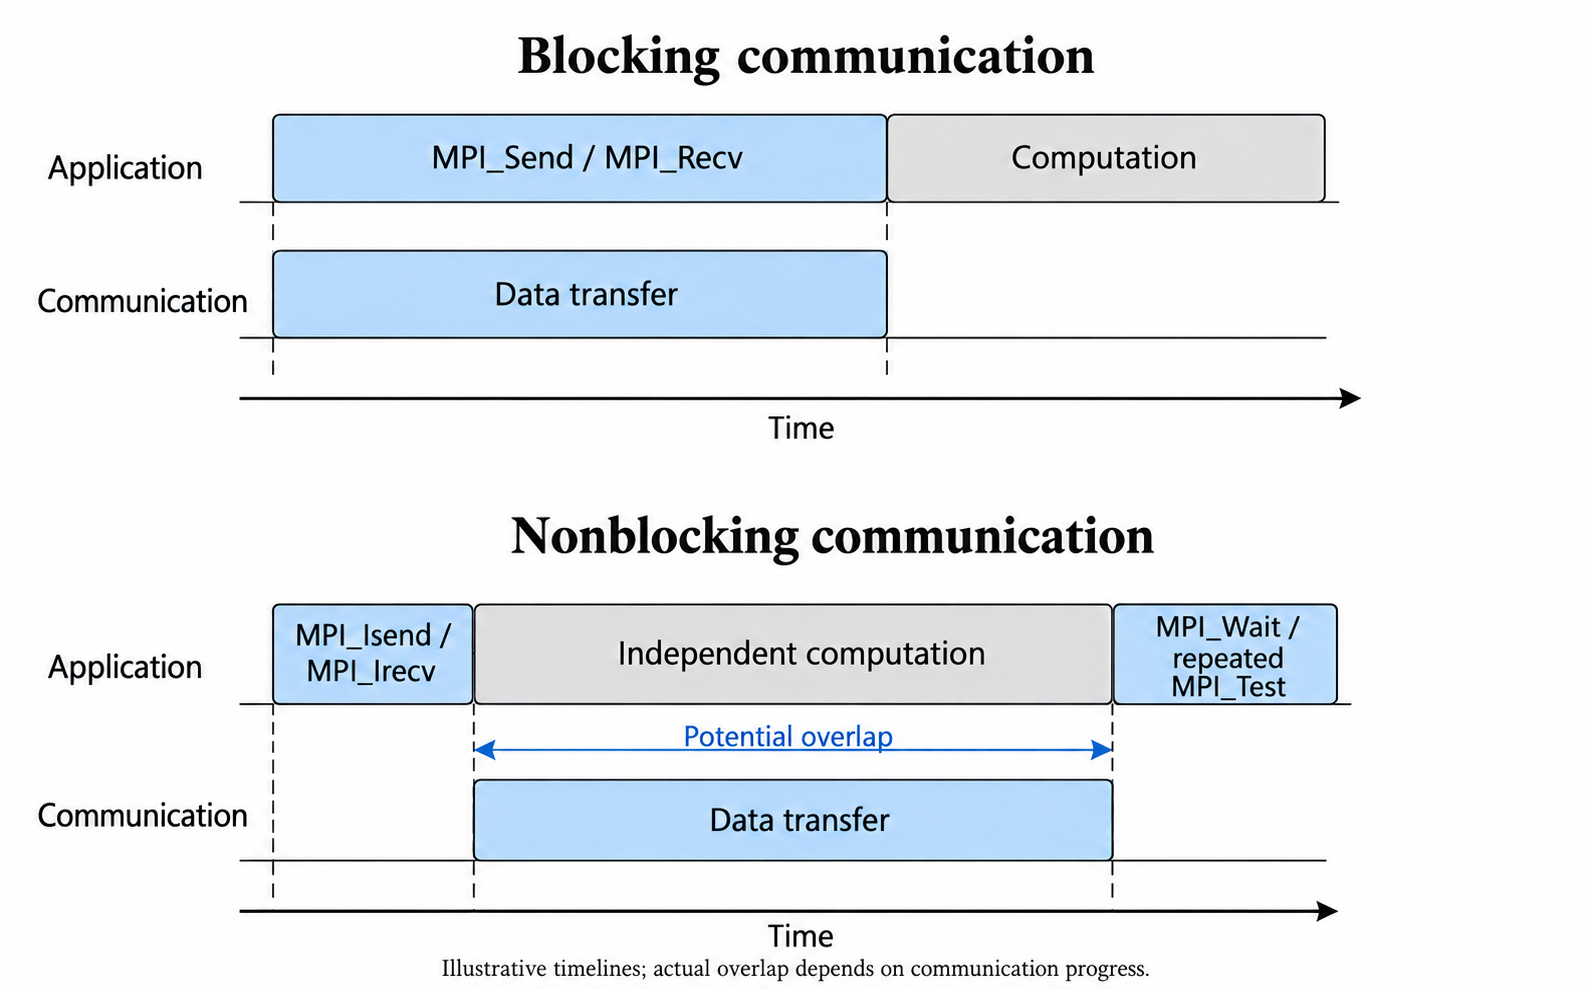
\includegraphics[width=0.9\textwidth]{figures/block_nonblock.png}
    \caption{Schematic comparison of blocking and nonblocking MPI
    point-to-point communication. Nonblocking operations separate
    initiation from completion, allowing independent computation
    to potentially overlap with communication. Actual overlap
    depends on communication progress during computation.
    The timelines are illustrative and not to scale.}
    \label{fig:blocking-nonblocking}
\end{figure}

As illustrated in \autoref{fig:blocking-nonblocking}, this separation
between initiation and completion creates a potential interval
in which independent computation can be performed while communication is
outstanding. Nonblocking communication therefore provides the programming
structure required for communication--computation overlap. However, it does not by itself guarantee that communication actually progresses while the application is performing computation without invoking communication or completion routines; this depends on the progress semantics and progress mechanisms of the MPI implementation~\cite{denis2016mpi}.



\subsection{Asynchronous Progress Mechanisms}

Asynchronous progress typically applies to nonblocking communication operations that have been initiated but not yet completed. For example, after communication has been initiated through \texttt{MPI\_Isend} and \texttt{MPI\_Irecv}, the corresponding requests may remain incomplete while the application thread continues executing computation~\cite[Sec.~4.7]{mpi50}. Progress on these communication operations can either be assisted explicitly by the application or provided independently by the MPI implementation. Asynchronous progress refers to the latter case and aims to decouple communication progress from application-level polling so that communication can continue to advance while the application thread performs computation~\cite{ruhela2019async}.

A common software-based mechanism is the use of one or more dedicated progress threads. These threads execute independently of the application thread and can advance communication operations that have not yet completed while application computation continues. Depending on the MPI implementation, their responsibilities may include request processing, protocol progression, and interaction with the underlying communication layer~\cite{ruhela2019async}. Asynchronous progress can also be partially supported by network hardware, for example through communication offload to the network interface, although the available mechanisms depend on the MPI implementation and its underlying communication stack~\cite[Sec.~3.9]{mpi50}.

Software progress threads consume processor resources, and their performance benefit therefore depends on CPU-resource allocation. A study of MPI nonblocking collectives on manycore processors has shown that progress-thread placement and the use of dedicated processor cores can affect the performance benefit obtained from communication--computation overlap~\cite{denis2019progressThreads}. If a progress thread shares processor resources with an application thread, additional resource contention and runtime overhead may be introduced~\cite{ruhela2019async}. Assigning dedicated CPU resources to progress can reduce such contention, but it also reduces the processor resources available for application computation. Consequently, enabling asynchronous progress does not necessarily improve overall performance; its effectiveness depends on whether the additional communication progress obtained during computation outweighs the corresponding resource consumption and runtime overhead~\cite{ruhela2019async}.


\subsection{Polling-Based Progress with \texttt{MPI\_Test}}

Another way to facilitate the progress of nonblocking communication is to periodically invoke nonblocking completion-test routines during computation. Functions such as \texttt{MPI\_Test} and \texttt{MPI\_Testall} check whether one or more communication requests have completed. If the corresponding operations are still incomplete, these routines do not block in the same way as \texttt{MPI\_Wait}, but instead return the current completion status. The application can therefore continue computation between polling points while periodically checking the state of the communication requests. MPI also defines progress requirements for repeatedly invoked test procedures, making these calls explicit opportunities for the implementation to advance communication operations that have not yet completed~\cite[Secs.~3.9, 4.7.3--4.7.5]{mpi50}.

When the application thread rarely enters MPI during computation and communication does not progress sufficiently on its own, periodic polling can improve communication--computation overlap. A typical approach divides the computation phase into smaller blocks and inserts completion tests between these blocks. If communication has not yet completed, execution returns immediately to computation and the requests are tested again at a later polling point. In this way, communication progress is assisted by periodic MPI test calls made by the application thread rather than relying on an independent asynchronous progress mechanism~\cite{mpiProgressGuidelines}.

The effectiveness of polling depends on the polling frequency. More frequent tests provide additional opportunities for communication progress and may reduce the amount of communication remaining at the final completion stage. However, each polling operation also consumes execution time and interrupts continuous computation. Excessively frequent polling can therefore introduce additional runtime overhead, whereas polling too infrequently may provide insufficient opportunities for communication progress. The polling frequency consequently represents a trade-off between communication advancement and the overhead introduced by the polling operations~\cite[Sec.~2.4]{zhou2024mpiProgressForAll}.

In this work, polling-based progress is evaluated separately from asynchronous progress. Nonblocking completion tests are periodically inserted into the computation interval to provide explicit progress opportunities, while computation continues between polling points. This makes it possible to distinguish application-assisted communication progress from asynchronous progress provided independently by the MPI implementation.



\section{MPI Implementations and Communication Stacks}

An MPI program uses the standardized MPI point-to-point interface regardless
of the underlying implementation~\cite{mpi50}. Internally, however, communication
passes through implementation-specific framework layers before reaching
shared memory or a network transport~\cite{intelFabricsControl,openmpiNetworkArchitecture,mpichDeveloperGuide}.
These layers select communication paths according to factors such as peer locality,
available devices, and runtime configuration.

In the implementations considered in this work, intra-node communication
generally uses a shared-memory path, whereas inter-node communication is routed
through a network module and ultimately a transport such as TCP or verbs
~\cite{intelFabricsControl,openmpiNetworkArchitecture,mpichDeveloperGuide}.
Consequently, comparisons between MPI implementations may also reflect
differences in internal communication frameworks and selected transport paths
unless these factors are controlled explicitly.

\autoref{tab:mpi-stacks} summarizes the principal layers relevant to
this study. It shows architectural alternatives rather than implying that all
paths are active in one execution. The exact versions and selected paths used
in the experiments are given in \autoref{chapter:methodology}.

\begin{table}[htbp]
    \centering
    \caption[Conceptual communication-stack layers of the evaluated MPI implementations.]{Conceptual communication-stack layers of the evaluated MPI
    implementations, based on the respective implementation documentation
    \cite{intelOfiProviders,openmpiNetworkArchitecture,mpichDeveloperGuide}.}
    \label{tab:mpi-stacks}
    \begin{tabular}{llll}
        \toprule
        Implementation & Framework layer & Intra-node path & Inter-node path \\
        \midrule
        Intel MPI & fabric selection & shared memory & OFI \\
        Open MPI & PML / BTL & self / vader BTL & TCP BTL or UCX/MTL \\
        MPICH & CH4 device & SHM module & OFI or UCX netmod \\
        \bottomrule
    \end{tabular}

    \vspace{0.3em}
\end{table}
\subsection{Intel MPI}

Intel MPI separates local and remote communication through its fabric
selection. The shared-memory fabric handles ranks on the same node. Inter-node
communication enters the Open Fabrics Interfaces (OFI) layer and then
libfabric, whose selected provider determines the concrete transport~\cite{intelFabricsControl,intelOfiProviders}. A TCP
provider uses the operating system's TCP and IP network stack, whereas a verbs provider
accesses InfiniBand or RoCE through the verbs interface. Provider selection
therefore changes the network path without changing the benchmark's MPI calls~\cite{intelOfiProviders}.

\subsection{Open MPI}

Open MPI uses a Point-to-Point Messaging Layer (PML) to coordinate MPI
point-to-point requests. With the \texttt{ob1} PML, data movement is delegated
to Byte Transfer Layers (BTLs): \texttt{self} handles communication with the
same process, \texttt{vader} handles shared-memory communication between local
processes, and \texttt{tcp} handles remote peers over TCP/IP~\cite{openmpiNetworkArchitecture,openmpiTcpFaq}. Other Open MPI
configurations may instead select the \texttt{ucx} PML, or the \texttt{cm} PML
with a Matching Transport Layer (MTL), but these form different communication
paths and must not be conflated with \texttt{ob1}/TCP measurements~\cite{openmpiNetworkArchitecture}. PML and BTL
selection also does not by itself imply the presence of a dedicated
asynchronous progress thread~\cite{openmpi418TcpProgress}.

\subsection{MPICH}

MPICH's CH4 device separates communication into a shared-memory module (SHM)
and a network module (netmod). Local peers can use the SHM path, while remote
communication is routed through a netmod such as OFI or UCX~\cite{mpichDeveloperGuide}. With the OFI
netmod, libfabric provider selection again determines whether the underlying
inter-node path uses TCP, verbs, or another supported fabric. Thus, CH4:OFI
identifies the MPI-to-libfabric architecture but does not uniquely identify
the physical network transport; the provider must also be reported~\cite{mpichDeveloperGuide,intelOfiProviders}.


\section{Related Work}
\label{sec:related-work}

Benchmarking communication--computation overlap requires more than measuring
communication latency or bandwidth in isolation. Denis and
Trahay~\cite{denis2016mpi} developed a benchmark suite for nonblocking
point-to-point communication and compared overlap across MPI libraries and
hardware platforms. Their use of different computation scenarios and
low-level traces illustrates how implementation behavior affects the overlap
observed by an application. This provides a methodological basis for
examining overlap through controlled benchmark experiments.


Research on progress mechanisms provides further context for interpreting
benchmark results. Schafer et al.~\cite{schafer2021exampiProgress} evaluated
strong progress in ExaMPI, including its ability to overlap communication
with computation without additional application MPI calls. Ruhela et
al.~\cite{ruhela2019async} developed a thread-based asynchronous progress
design that avoids dedicated processor resources and reduces interference
from thread scheduling. These studies investigate progress-engine designs;
the present thesis instead evaluates the progress configurations available
in the installed MPI implementations on the test system.

Zhou et al.~\cite{zhou2024mpiProgressForAll} analyzed the ambiguity of MPI progress and pointed out that nonblocking operations do not by themselves guarantee continuous progress between initiation and completion. They discussed two common approaches for providing progress during computation: explicit polling with \texttt{MPI\_Test} and background progress threads, including the overheads associated with both approaches. They further proposed interfaces for explicitly managing MPI progress.



At the application level, Mittermair et al.~\cite{mittermair2025automatic} studied automatic distributed parallelization of structured-grid stencil kernels for ocean-modeling applications. Their approach derives the required halo communication by analyzing data dependencies and automatically inserts the corresponding communication operations into the generated distributed code. Their work shows, at the application level, how halo communication requirements can be derived from the data dependencies of stencil computations, providing relevant background for the present thesis. This thesis focuses on a different question at the runtime level: when a computation window exists between the initiation and completion of nonblocking communication, how outstanding communication progresses under different MPI configurations and how much communication--computation overlap can ultimately be observed.

The focus of this thesis is a benchmark-based evaluation on the LRZ
CoolMUC-4 system. Using an extended Comb benchmark, it investigates how
MPI implementation, transport configuration, peer payload, and progress
settings affect measured overlap in this environment. The experiments
also examine completion methods, computation-window duration, and explicit
polling during computation. The contribution is an empirical assessment
of these choices under the tested configurations, rather than a new MPI
progress algorithm. Its findings characterize this benchmark and system;
application-level speedups for a complete ocean model require separate
validation.
